\documentclass{report}

\usepackage[english]{babel}
\usepackage[utf8]{inputenc}

\usepackage{amsmath}
\usepackage{graphicx}
\usepackage{hyperref}
\usepackage{geometry}

\hypersetup{
colorlinks  = true,
linkcolor   = black,
urlcolor    = red,
}

\newgeometry{
      top = 0.75in,
      bottom = 0.75in,
      left = 0.75in,
      right = 0.75in,
}

\title{Activity Bot's Catch Game\\
\Large{University of Maribor}}

\author{Bruno Silva}

\setcounter{chapter}{1}

\begin{document}
\maketitle

\chapter*{Abstract}
Your abstract. 

\tableofcontents

\section{Introduction}

\section{Some examples to get started}

\subsection{How to create Sections and Subsections}


\subsection{How to include Figures}




\begin{figure}
\centering
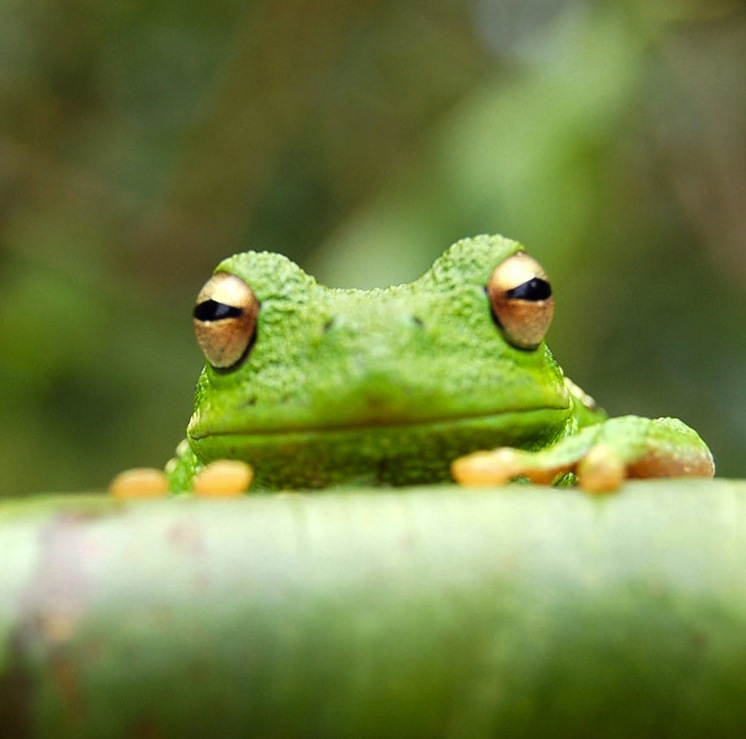
\includegraphics[width=0.3\textwidth]{resources/frog.jpg}
\caption{\label{fig:frog}This frog was uploaded via the file-tree menu.}
\end{figure}

\bibliographystyle{alpha}
\bibliography{sample}

\end{document}